\chapter{Multi-commodity problem}

On a graph $G = (V,E)$ and $k$ tuples $(s_{1}, t_{1}), (s_{2}, t_{2}), \dots, (s_{k}, t_{k}) \ in V^{2}$ known as \textbf{commodities} we can also define a network and a flow. Same as before we have a capacity $c: E \to \R_{0}^{+}$. These commodities are shared on the same resources.

We may define $\mathcal{P}_{i}$ as all paths between $s_{i}$ and $t_{i}$. And also $\mathcal{P} := \bigcup_{i = 1}^{k} \mathcal{P}_{i}$.

For a single commodity flow problem we could define an \textit{linear program} (LP):

$$
\begin{array}{rl}
	& \max \sum_{p \in \mathcal{P}_{st}} f_{p} \\
	\forall e \in E & \sum_{p: e \in p \in \mathcal{P}_{st}} f_{p} \leq c(e) \\
	& f \geq 0
\end{array}
$$

From this we may define an linear program denoted as \textbf{LP1} for multi commodity problem.

$$
\begin{array}{rl}
	& \max \sum_{p \in \mathcal{P}} f_{p} = \sum_{i = 1}^{k} \sum_{p \in \mathcal{P}_{i}} f_{p} \\
	\forall e \in E & \sum_{j = 1}^{k} \sum_{p: e \in p \in \mathcal{P}_{j}} f_{p} \leq c(e) \\
	& f \geq 0
\end{array}
$$

Alternatively we could define it by a single variables for flows on each edge. For multi commodity problem we would have $k$ flows which adds up to one single flow. Thus we can see that the problem is in $P$ (polynomial).

\section{Multi cut problem}

As a cuts for single flow we may define somewhat similiar definition. Such that between every tuple of $s_{i}$ and $t_{i}$ there is no such path. We will also look at a linear program which will be denoted as \textbf{LP2}.

$$
\forall e : x_{e} =
\left\{
\begin{array}{rl}
	1 & e \text{ in cut} \\
	0 & \text{otherwise}	
\end{array}
\right.
$$

$$
\begin{array}{rl}
	\Phi := & \min \sum_{e \in E} x(e) c(e) \\
	\forall i \in [k] \forall p \in \mathcal{P}_{i} & \sum_{e \in p \in \mathcal{P}_{i}} x(e) \geq 1 \\
	\text{(ILP)} & x(e) \in \{0, 1\} \\
	\text{(LP)} & x(e) \geq 0
\end{array}
$$

First ILP is integer linear program which is generally NP hard. Thus we will look on the relaxation of LP program. We may observe that we don't need to specify that $x(e) \geq 1$.

Now we may see that indeed \textbf{LP1} and \textbf{LP2} are dual programs. Thus resulting in knowing that the maximum flow is the same as minimum fractional cut.

\section{Example}

Before we continue we will take a look at a simple example (\ref{example}). The graph is as follows. All capacities are equal to $1$.

\begin{figure}[!h]\centering
	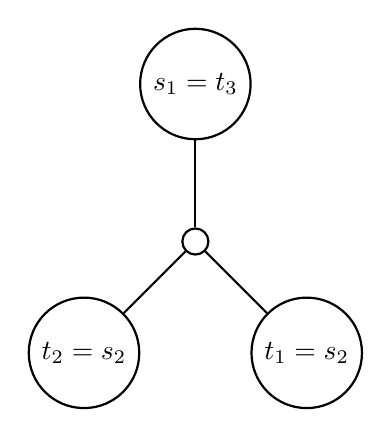
\begin{tikzpicture}[node distance={20mm}, thick, main/.style = {draw, circle}]
		\node[main] (1) {$s_{1} = t_{3}$};
		\node[main] (4) [below of=1] {};
		\node[main] (2) [below right of=4] {$t_{1} = s_{2}$};
		\node[main] (3) [below left of=4] {$t_{2} = s_{2}$};
		\draw (1) -- (4);
		\draw (4) -- (2);
		\draw (4) -- (3);
	\end{tikzpicture}
	\caption{Example graph.}
	\label{example}
\end{figure}

We may observe that the max flow is $|f| = \frac{3}{2}$ because we can put $\frac{1}{2}$ on every edge. Then multi-cut is $2$ since we need to remove always at least two edges. But minimum fractional multi-cut is only $\frac{3}{2}$ because we only have to "cut" half of each edge. Thus it is the exact same result as max flow.

\section{Preparation for algorithm}

We will show an algorithm which will give an approximate result of a multi-cut problem. We may look at it like we would cut off some parts of the graph which are close to the sources and continue.

Given $\bar{G} = (\bar{V}, \bar{E}), (s_{i}, t_{i}), k, c: E \to \R_{0}^{+}$ and solution $x$ of \textbf{LP2}. We define:

$$
B_{x}(s_{i}, r) := \{u \in \bar{V} | d_{x} (s_{i}, u) \leq r\}
$$

As a ball around $s_{i}$ with diameter w.r.t $x$. $d_{x} (s_{i}, u) :=$ the length of the shortest $s_{i}u$ path in $\bar{G}$ w.r.t. the edge length $x(e)$.

$$
\delta (B_{x}(s_{i}, r)) = \{\{u,v\} \in \bar{E} : |\{u,v\} \cap B_{x}(s_{i}, r)| = 1\}
$$

$$
V_{x}(s_{i}, r) = \frac{\Phi}{k} + \sum_{\{u,v\} \in \bar{E}, u,v \in B_{x}(s_{i},r)} c(e)x(e) + \sum_{\{u,v\} \in \delta(B_{x}(s_{i},r)): u \in B_{x}(s_{i},r)} c(e) (r - d_{x}(s_{i}, u))
$$

This we call a volume of a ball. We will denoted as a function of $r$ $f(r)$. The last sum is of all edges which are only partly inside the ball. Next we also define the following.

$$
C_{x}(s_{i}, r) = \sum_{\{u,v\} \in \delta(B_{x}(s_{i},r))} c(u,v)
$$

This will be denoted as a function $g(r)$. We may see some really nice properties these functions have. For instance $f(r)$ is a growing function which is increasing linearly and then it jumps to another point. On the other hand $g(r)$ is constant at some parts and then it jumps to a certain point, these jumps are for both function in the exact same spots. Next we can see that for some nice points it holds that $f'(r) = g(r)$.

\begin{lemma}
	For each $i \in [n]$ s.t. $s_{i}, t_{i} \in \bar{V}$ there exist $r \in (0, 1/2)$ s.t.
	
	$$
	\frac{C_{x}(s_{i}, r)}{V_{x}(s_{i},r)} \leq 2 \ln 2k.
	$$
\end{lemma}

\begin{myproof}
	By contradiction. For fixed $i$ $\forall r \in (0, 1/2)$, $\frac{f'(r)}{f(r)} > 2 \ln 2k$. We will have $r_{0} = 0 < r_{1} < r_{2} < \dots < r_{l-1} < 1/2 = r_{l}$ which are the values where $f(r)$ is not continuous (there are these "jumps"). First we consider $(r_{j}, r_{j+1})$ for some $j$.
	
	$$
	\frac{f'(r)}{f(r)} = \left( \ln f(r)\right)'
	$$
	
	So $\forall r \in (r_{j}, r_{j+1})$, $\left( \ln f(r)\right)' > 2 \ln 2k$. We will compute the integral over all of these values. We may see that the right side is just a constant so we get
	
	$$
	\int_{r_{j}}^{r_{j+1}} \left( \ln f(r)\right)' > (r_{j+1} - r_{j}) 2 \ln 2k.
	$$
	
	In $r_{j+1}$ there may be jump so we instead take the $\lim_{r \to r_{j+1}^{-}} f(r) = f^{-}(r_{j+1})$. Note that $f^{-}(r_{j+1}) \leq f(r_{j+1})$.
	
	$$
	\ln f(r_{j+1}) - \ln f(r_{j}) \geq \ln f^{-}(r_{j+1}) - \ln f(r_{j}) = \int_{r_{j}}^{r_{j+1}} \left( \ln f(r)\right)' > (r_{j+1} - r_{j}) 2 \ln 2k.
	$$
	
	Now we sum our inequality over all intervals $(r_{j}, r_{j+1}), j = 0, \dots, l$. We will only have the very ends because the rest will be once added and once removed.
	
	$$
	\sum_{j = 0}^{l-1} \left( \ln f(r_{j+1}) - \ln f(r_{j}) \right) > \sum_{j = 0}^{l-1} (r_{j+1} - r_{j}) 2 \ln 2k
	$$
	
	$$
	\ln f(r_{l}) - \ln f(r_{0}) > (r_{l} - r_{0}) 2 \ln 2k
	$$
	
	$$
	\ln f(1/2) - \ln (0) > \ln 2k
	$$
	
	$$
	\ln \frac{f(1/2)}{\frac{\Phi}{k}} > \ln 2k
	$$
	
	$$
	\frac{f(1/2)}{\frac{\Phi}{k}} > 2k
	$$
	
	$$
	f(1/2) > 2 \Phi
	$$
	
	As the volume of the entire pipe system is at most $2 \Phi$ it means that we have a contradiction.
\end{myproof}

Note that choosing $1/2$ is not necessary for the proof, but for the algorithm to work. Because if we choose $1/2$ it means that no $s_{j}, t_{j}$ will both be in a ball for the index $i$. That is because the length w.r.t $x$ of paths from $s_{j}$ to $t_{j}$ need to be at least $1$.

\section{Pipe cut algorithm}

\begin{algorithm}[!h]
	\caption{Pipe cut algorithm}
	\begin{algorithmic}[1]
		\Require $\bar{G} = (\bar{V}, \bar{E})$.
		\Ensure $F$ multi cut.
		\State $F \gets \emptyset$
		\For{$i = 1 \dots k$}
			\If{$s_{i}-t_{i}$ are still connected in $(\bar{V}, \bar{E} \setminus F)$}
				\State Choose $r \in (0, 1/2)$ by Lemma.
				\State $F \gets F \cup \delta(B_{x}(s_{i}, r))$
				\State Remove edges inside $B_{x}(s_{i}, r)$ and $\delta(B_{x}(s_{i}, r))$.
			\EndIf
		\EndFor \\
		\Return $F$
	\end{algorithmic}
\end{algorithm}



There are few things to talk about. To get $r$ we will check all "almost ends" of all intervals. The time complexity is polynomial since everything that is inside the code is polynomial. Correctness of the algorithm is easily observable since no pair $p_{i},t_{i}$ is inside some other ball and all balls will separate pairs $s_{j}, t_{j}$. Other thing to consider is what is the approximation ratio?

\begin{thm}
	Approximation ratio of the Pipe cut algorithm is $O(\log k)$.
\end{thm}

\begin{myproof}
	Lets define $C_{i}$ as the cost of the cut of the ball from iteration $i$ and $V_{i}$ as the volume of it. We know that $C_{i} \leq 2 \ln 2k \cdot V_{i}$.
	
	$$
	\sum_{i} C_{i} \leq 2 \ln 2k \sum_{i}V_{i} \leq 2 \ln 2k \cdot 2 \Phi = 4 \ln 2k \cdot \Phi = O (\log k) \Phi
	$$
\end{myproof}

For a single commodity we know that max flow $=$ min cut. Where $\leq$ is trivial and $\geq$ is a little harder. This is a case of \textbf{exact duality}. On the other hand we already shown that this doesn't hold for multi-commodity, but what if we can define \textbf{approximate duality}.

\begin{cor}
	Max flow $\leq$ min cut $\leq O(\log k)$ max flow. For multi-commodity.
\end{cor}

\begin{myproof}
	Because of the duality of LP1 and LP2 we know that max flow is the same as min fractional multi-cut. And because of the algorithm we know that the fractional multi-cut is in $O(\log k)$.
\end{myproof}

\section{How to solve LP}

There is still a problem with our LP which can have up to exponential many of constraints. But this can be solved fast by using \textbf{Ellipsoid algorithm} on $A x \leq b$. Only think it needs is an so called \textbf{ORACLE} which is that for given $\bar{x}$, check whether $A\bar{x} \leq b$ and if not return a violated constraint.

In our case \textbf{ORACLE} is for each $i$ find the shortest $s_{i}-t_{i}$ path w.r.t $\bar{x}$. This can be either $1$ and we are happy or $< 1$ then this constraint is violated.

\section{Is there any better approximation?}

We will show that indeed this approximation is the best we can get. Firstly we will define a new property of graphs.

A graph $G = (V,E)$ is an \textbf{$\alpha$-expander} if $\forall S \subseteq V, |S| \leq \frac{n}{2}, \delta(S) \leq \alpha |S|$.

We take as granted that it holds: $3$-regular $\alpha$-expanders exist for $\alpha > 0$. Now lets observe (\ref{3-regular})that at most $1 + 3 \cdot 2^{l-1}$ vertices are reachable by a path of length $\leq l$.

\begin{figure}[!h] \centering
	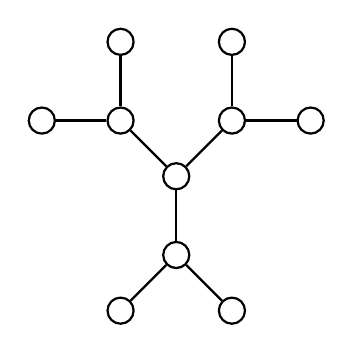
\begin{tikzpicture}[node distance={10mm}, thick, main/.style = {draw, circle}]
		\node[main] (1) {};
		\node[main] (2) [below of=1] {};
		\node[main] (3) [above right of=1] {};
		\node[main] (4) [above left of=1] {};
		\node[main] (5) [below left of=2] {};
		\node[main] (6) [below right of=2] {};
		\node[main] (7) [above of=3] {};
		\node[main] (8) [right of=3] {};
		\node[main] (9) [above of=4] {};
		\node[main] (10) [left of=4] {};
		\draw (1) -- (4);
		\draw (1) -- (2);
		\draw (1) -- (3);
		\draw (2) -- (5);
		\draw (2) -- (6);
		\draw (3) -- (7);
		\draw (3) -- (8);
		\draw (4) -- (9);
		\draw (4) -- (10);
	\end{tikzpicture}
	\caption{How to get the upper bound.}
	\label{3-regular}
\end{figure}

If we take $l = \log_{2} \frac{n-2}{6} + 1$ so with the upper bound we get $1 + 3\frac{n-2}{6} = 1 + \frac{n-2}{2} = \frac{n}{2}$. And also we define an instance of multi-commodity problem: $T = \{\{u,v\} | \delta(u,v) > l\}$. A unit of flow consumes $\geq l$ units of volume of the entire system. Thus $|E| = O(n)$. Therefore max flow $\leq O(\frac{n}{l}) = O(\frac{n}{\log n})$. But for min cut we take the optimum $F \subseteq E$. Every path in $G = (V, E \setminus F)$ is $\leq \frac{n}{2}$ so min cut os $\Theta(n)$. Thus it is indeed tight.